\section{Graphische Benutzungsoberflächen - Kontrollfragen}
\subsection{Begriffe und Geschichte}
\begin{enumerate}
	\item Erläutern Sie die Begriffe Dialogsystem, UI und Usability!
	\begin{itemize}
		\item \textbf{Dialogsystem}: auch interaktives System. Kombination von Hardware- und Softwarekomponenten, die Eingaben vom Benutzer empfangen und Ausgaben zum Benutzer übermitteln, um ihn bei der Ausführung einer Arbeitsaufgabe zu unterstützen
		\item \textbf{UI - Benutzungsschnittstelle} Alle Bestandteile eines interaktiven Systems, die Informationen und Steuerelemente zur Verfügung stellen, die für den Benutzer notwendig sind, um eine bestimmte Arbeitsaufgabe mit dem interaktiven System zu erledigen. 
		\item \textbf{Usability} Das Ausmaß, in dem ein Produkt durch bestimmte Benutzer in einem bestimmten Nutzungskontext genutzt werden kann, um bestimmte Ziele effektiv (effectiveness), effizient (efficienty) und zufriedenstellend (satisfaction) zu erreichen.
	\end{itemize}
	
	\item Welche Schnittstellen hat ein Dialogsystem?
	\begin{itemize}
		\item Benutzungsschnittstelle (UI)
		\item Applikationsmodule
		\item Grundprinzip: UI fragt nach Eingabe -> gibt Eingabe an Appl.Module -> Rückgabe der unformatierten Ausgabe an UI -> UI gibt formatierte Ausgabe an Nutzer
	\end{itemize}
	\begin{figure}[!h]
		\centering
		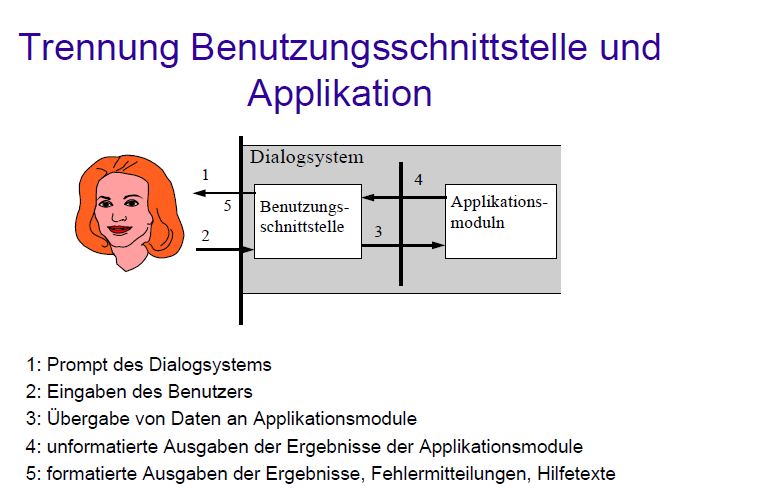
\includegraphics[scale=0.5]{img/ui.png}
	\end{figure}
	
	\item Welche Modelle muss ein Dialogautor beim Entwurf von Benutzungsschnittstellen beachten?
	\begin{itemize}
		\item Benutzermodell -> mentales Modell \\
		Aspekte des Modells: Anwendungsbereich, Arbeitsaufgabe/kontext, kenntnisse, Erfahrungen, Fertigkeiten
		\item Aufgabenmodell -> hauptsächlich HCI im Fokus
		\item Architekturmodell -> UI-Software
		\item Dialogspezifikationsmodell -> siehe Frage vorher(?)
	\end{itemize}
	
	\item Welche Beiträge kann die Ergonomie zur Erstellung von Benutzungsschnittstellen leisten?
	\begin{itemize}
		\item Optimieren der Arbeitsabläufe durch niedrigen Aufwand des Benutzers und hohe Funktionalität des Dialogsystems
		\item ganzheitliche Gestaltung der Software
		\begin{itemize}
			\item benutzergerecht: Berücksichtigung der Stärken und Schwächen des Menschen
			\item aufgabenangemessen: Computer werden vom Benutzer zur Bearbeitung konkreter Aufgaben eingesetzt
			\item technikbewusst: neue technische Optionen zum Wohle des Benutzers einsetzen
			\item organisationsgerecht: Berücksichtigung der organisatorischen Einbindung
		\end{itemize}
		\item Computerwissenschaften -> Softwaredesign -> Dialogtechniken (Informationsdarstellung, Ablauf,..), Software Engineering (Analyse, Modellierung, Entwurf,..), 
		\item Arbeitswissenschaften -> Arbeitsplatzgestaltung; Arbeitspsychologie
		\item Humanwissenschaften -> Physiologie
		\item Psychologie -> Kognition (Gedächtnis, Verstehen, Lernen); Wahrnehmung 
		\item Ergebnisse der Ergonomie:
		\begin{enumerate}
			\item Gesetze und Verordnungen zum Arbeitsschutz
			\item Normen ((inter-)nationale Standards)
			\item Empfehlungen
			\item Designregeln (Gestaltungsregeln, Style Guides, Pattern)
			\item Tools 
		\end{enumerate}
	\end{itemize}
\end{enumerate}


\subsection{Modelle der Human-Computer-Interaction}
Es gibt nicht ein Gesamtmodell, sondern viele Teilmodelle, die in
unterschiedlichen Aspekten hilfreich sein können.
\begin{enumerate}
	\item Was ist ein Dialogsystem?
	siehe subsection vorher
	
	\item Was ist die Benutzungsschnittstelle/User Interface?
	siehe subsection vorher
	
	\item Welche Schnittstellen hat ein Dialogsysteme?
	siehe subsec vorher
	
	\item Welche Modelle müssen Dialogautoren beachten, Welche Rollen gibt es?
	\begin{itemize}
		\item Modelle siehe subsection vorher
		\item Gestalter und Bewerter der physischen Umgebung
		\item Entwickler von UI Tools
		\item Enwickler von UI /Dialogautor
		\item Designer
		\item Bewerter von UI
		\item Applikationsanalysator
		\item Applikationsprogrammierer
		\item ...
		\item Endbenutzer
	\end{itemize}
	
	
	\item Was ist das Seeheim-Modell?
	\begin{itemize}
		\item (ähnlich MVC)
		\item 3 Bestandteile: \\
		Presentation (lexikalische Ebene): für systemnahe Ein/Ausgaben zuständig; verfügt dazu über Devices=Schnittstellen zu physikalischen oder logischen (zb Menüs) Ein/Ausgabegeräten\\
		Dialog control (syntaktische Ebene): durch Austausch von Token Ablauf des Dialogs regeln; unabhängig von Geräte und Anwendung\\
		Applicaiton interface (semantische Ebene): Vermittlerrolle zw. Dialogcontrol und Applikation
		\item Grenzen: Wie erfolgt der Kontrollfluss (siehe nächste Frage)? von welcher Art ist die Kommunikation? (Nachrichtenaustausch oder Prozeduraufruf?)\\
		''schnelle'' grafische Ausgaben brauchen ''Sonderwege'' (wtf?)
	\end{itemize}	
	\begin{figure}[!h]
		\centering
		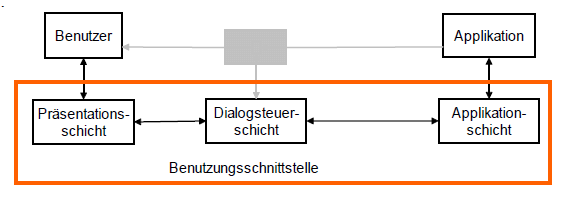
\includegraphics[scale=0.5]{img/seeheim.png}
		\caption{Seeheim Model}
	\end{figure}
	
	\item Welche Vor- und Nachteile haben interne und externe Kontrollarchitekturen
	im Seeheim-Modell?\\
	\textbf{intern:} Programm besitzt alleinige Kontrolle über UI; UI steht als Paket von Unterprogrammen zur Verfügung\\
	\textbf{extern:} Anwendung in Unterprogramme unterteilt, welche von UI aufgerufen werden\\
	\begin{table}[!h]
		\centering
		\begin{tabular}{|p{10em}|p{15em}|p{15em}|}
			\hline
			\hline
			& \textbf{Vorteile} & \textbf{Nachteile}\\
			\hline			
			\textbf{intern} & \tabitem einfache Realisierung & \tabitem keine saubere Aufgabentrennung\\
			&	\tabitem optimale Anpassung an das Anwendungsprogramm & \tabitem bei Änderung an der UI Eingriffe im gesamten Programm\\
			& \tabitem entspricht Vorgehensweise bei Systementwicklungen und Aufgabenzerlegungen & \tabitem sehr lokale Dialoge \\
			&& \tabitem Einheitlichkeit und Konsistenz der UI hängen von Programmierdisziplin ab \\
			\hline
			\hline
			\textbf{extern} &  \tabitem saubere Separierbarkeit von UI und Anwendungsfunktionalität & \tabitem Anwendungsprogramme müssen atomierbar sein\\
			& \tabitem benutzerspezifische UI lässt sich angemessen realisieren & \tabitem Dynamik/Interaktionsfolge liegt außerhalb der Anwendung\\
			& \tabitem anwendungsunabhängige Modifizierbarkeit & Verteilung der Semantik\\
			& \tabitem Leichte Portierbarkeit vom Prototyp zur fertigen Anwendung & \tabitem Komplexität der Schnittstellenbeschreibung\\
			&& \tabitem mögliche Redundanzen in den verschiedenen Unterprogrammen\\
			&& \tabitem Ausgabeaufforderung der Anwendung\\
			\hline
		\end{tabular}
		\caption{Vor- und Nachteile der Kontrollarchitekturen im Seeheim-Modell}
	\end{table}
	
	\item Nennen sie Modelle für Dialogspezifikationen!\\
	dienen zur formalen Spezifikation des Dialogablaufs\\
	sollen ausdrucksstark und einfach sein; typische Dialogstrukturen unterstützen (parallele Prozesse, sequentielle Schritte, Verzweigungen des Ablaufs); unterschiedliche Detailstufen
	\begin{itemize}
		\item Multi-Party-Grammatiken: kontextfreie Grammatiken; Erweiterung der BNF durch Spezifikation wer was tut bei Interaktion; einfach und natürlich, aber nicht ausdrucksstark
		\item Menühierarchien: baumartige Struktur zur Spezi von Alternativen; einfach, aber nicht ausdrucksstark
		\item Zustandsübergangsdiagramme (STN): quasi Graph der Transitionen darstellt
		\item verbesserte STN (=ATN)
		\item State Charts: lösen einige Probleme der STN/ATN, zb Hierarchische, nebenläufige, Zustände, History
		\item Ereignis Handler: Dialogbeschreibung durch Regeln
		\item Petri-Netze: sollte klar sein
		\item User-Action-Notation
	\end{itemize}
		
	\item Welche Benutzermodelle kennen sie?\\
	Ziel: konsistentes Dialogverhalten auch in breitem Anwendungsbereich anhand Wissen des Nutzers über Anwendungsbereich, seine Ziele und seine Pläne\\
	Einteilung nach Datenverarbeitungskenntnissen (DV):
	\begin{itemize}
		\item Anfänger
		\item gelegentlicher Nutzer
		\item Experte
	\end{itemize}
		
	\item Welche Benutzerklassen sollten unterschieden werden?\\
	Kriterien zur Unterscheidung von Benutzern
	\begin{itemize}
		\item \textbf{Vorwissen/Fachliche Erfahrung:} zum Anwendungsgebiet -> mit Erfahrung geht Anwender mit Erwartungen an neues Tool
		\item \textbf{Vertrautheit:} mit Begriffen und Konzepten der DV prägen das Verhalten beim Dialog
		\item \textbf{Kognitive Fähigkeiten:} Stil der Problemlösung, Experimentierfreudigkeit oder Ägnstlichkeit beschleunigen oder verzögern das Lernverhalten
		\item \textbf{Einstellungen:} ggüber Dialogsystemen können Effektivität beeinflussen -> grundsätzliche Haltung ggüber Computern; persönliche Gründe für das Arbeiten (freiwillig - zwang; privat - beruflich)
		\item \textbf{Persönliche Ziele:} beim Erlernen der Bedienung des Systems -> vorrangig ist Arbeitsaufgabe, Beherrschen der Systeme nur soweit wie nötig ODER primäres Ziel ist Verstehen und Beherrschen des Systems
	\end{itemize}
	
	\item Was sind Personas?\\	
	beschreiben fiktive Benutzer als Stereotyp und Referenzperson zur Analyse und Definition von Anforderungen an interaktive Systeme -> Stereotyp zwingt zum Nachdenken über konkrete statt allgemeine Nutzer
	
	\item Erläutern sie das Model-View-Controller- Modell!
	\begin{itemize}
		\item entstanden als Experiment aus Seeheim Modell
		\item Aufteilung in Klassen - MVC halt..
		\item Vorteile: problemlose Integration in OO Entwurf; problemlose Anpassung an unterschiedliche Benutzer; Unterstützung unterschiedlicher Sichten auf Daten
		\item Probleme: MVC als alleiniges Architekturmodell nicht geeignet; Trennung Ctrl - View oft nicht zweckmäßig
	\end{itemize}
	
	\item Wozu dienen GOMS-Modelle?
	\begin{itemize}
		\item \textbf{G}oals: eine Menge von Zielen
		\item \textbf{O}perators: Menge von Operationen
		\item \textbf{M}ethods: Menge von Methoden zum Erreichen von Zielen
		\item \textbf{S}election rules: Menge von Auswahlregeln von Methoden
		\item geht von geübten Nutzern aus, d.h. jene die das System bereits kennen
		\item Modell erlaubt Abschätzungen oder Vorhersagen des Lernaufwandes für den Erwerb des prozeduralen Benutzerwissens
		\item zusätzliche Vorhersagen für Ausführungsaufwand und Performanz 
		\item Kritik: Berücksichtigt nicht Ermüdung des Nutzers, soziales organisatorisches Umfeld, Unberechenbarkeit des Nutzers, Gewohnheiten/Vorlieben des Nutzers
	\end{itemize}
\end{enumerate}


\subsection{Wahrnehmung}
\begin{enumerate}
	\item Welche Prozesse spielen beim statischen und dynamischen Sehen eine Rolle?
	\begin{itemize}
		\item Statisches Sehen: Hell-Dunkel, Farbe, Scharf Sehen; nicht sehen
		\item dynamisches Sehen: Bewegungen; Peripheres sehen, Augenbewegungen
		\item Informationswahrnehmung
		\item Hell-Dunkel: Verantwortlich dafür Stäbchen im Auge -> erweiterbar durch Irisöffnung (schließen bei Helligkeit und vice-versa); Anpassung dauert Sekunden bis Minuten
		\item nichtSehen: blinder Fleck an Verbindung Sehnerv mit Netzhaut
		\item Farbe: elektromagnetische Wellen wahrnehmen\\
		unterschiedliche Sensibilität für verschiedene Farben
		\item Peripher Sehen: unscharfes Sehen in der Peripherie der Netzhaut; 
	\end{itemize}
	
	\item Wie erfolgt die Wahrnehmung von Objekten beim Menschen?
	\begin{itemize}
		\item Abbildung von 2D Helligkeitsverteilungen auf der Netzhaut in 3D Repräsentation von Objekten
		\item 80\% aller Informationen übers Auge zum Gehirn
		\item Objekte ohne Mühe wahrnehmen
		\item Entdecken von Signalen vor einem Rauschhintergrund
		\item Erkennen Szenen (komplexe Reizkonfiguration)
		\item Konzentration auf wesentliche Informationen
	\end{itemize}
	\item Nennen Sie Faktoren zur Erkennung räumlicher Tiefe!
	\begin{itemize}
		\item monokulare Faktoren: Größendistanz, Überdeckungen, Schattierungen, Helligkeit und Kontrast
		\item Bewegungsfaktoren: Bewegungsparallaxe (=scheinbare Bewegung eines Objektes, wenn man seine eigene Position verändert); kinematische Tiefeneindrücke
		\item binokulare Faktoren: Binokulraie Disparität -> sehen Bild mit jedem Auge, aber durch Entfernung leicht unterschiedlich -> Gehirn mischt daraus die Tiefeninformation
		\item okulomotorische Faktoren: Konvergenz (Drehung der Augen) -> Bsp: einwärts Drehen um dichte Objekte scharf zu stellen; Akkomodation (=Formveränderung der Linse)
	\end{itemize}
	
	\item Wie erkennen wir Text?
	\begin{itemize}
		\item Verarbeitung von 4 Zeichen links und 6 Zeichen rechts vom Fixationspunkt (europ. Raum)
		\item Außerhalb dieses Bereiches nur Wortmerkmale (Form, Trennzeichen, Umhüllung) zur Bestimmung des Fixationspunkts
		\item zeitliche Auflösung beim Lesen: 50 - 200ms
		\item nach Studie: wichtig sind nur erster und letzter Buchstabe; Reihenfolge der inneren egal -> Gehirn sortiert diese richtig
	\end{itemize}


	\item Erläutern Sie die Gestaltgesetze von Wertheimer!
	\begin{itemize}
		\item ''Das Ganze ist mehr als die Summe seiner Teile!''
		\item Prinzipien der Gestaltbildung: Ausnutzung strukturell informationstragender Teile (Wende-, Knick-, Krümmungspunkte), weglassen redundanter Teile
		\item Gesetze: 
		\item Figur und Grund: (-Trennung) helle, symmetrische, konvexe oder kleine Flächen zur Figur;\\
		dunkle, asymmetrische, konkave oder größere Flächen werden zum Hintergrund (oftmals)
		\item Gesetz der guten Form (Gestalt): Betrachter bildet Gruppen von Darstellungselemeneten aufgrund der Neigung zur Einfachheit, Regelmäßigkeit, innerem Gleichgewicht, Symmetrie und Geschlossenheit von Formen
		\item Gesetz der Ähnlichkeit: Tendenz zur Gruppierung von Darstellungselementen gleicher Art (Größe, Form, Farbe)
		\item Gesetz der Geschlossenheit: Objekte werden so wahrgenommen, dass sich eine einfache Interpretation ergibt
		\item Gesetz der Erfahrung/Erwartung: Bedeutungsinhalt hilft Figuren vom Hintergrund zu trenne
		\item Gesetz der Kontinuität
	\end{itemize}
	\item Was beinhalten die 3 Farbtheorie und die Gegenfarbtheorie?
	\begin{itemize}
		\item 3Farbtheorie: es existieren 3 Rezeptorsysteme für unterschiedliche spektrale Empfindlichkeit
		\item Gegenfarbtheorie: Gegensatzpaare: Rot-Grün; Blau-Gelb
	\end{itemize}
	
	\item Wie lässt sich Farbe beim Entwurf von Benutzungsschnittstellen einsetzen?
	\begin{itemize}
		\item Farben harmonieren oder erzeugen Disharmonie (erzeugt Ablehnung)
		\item Unterstützung der visuellen Informationsverarbeitung
		\item kann vom Nutzer als ästhetisch ansprechender, hilfreicher empfunden werden
		\item können subjektive Sicherheit erhöhen		
		\item Farbe unterstützt Kommunikation mit Empfänger, wenn Farbregeln des Anwendungsgebietes eingehalten werden
		\item bei gelungener Farbgestaltung: bessere Informationsverarbeitung
		\item Visualisieren von Zuständen/Übergängen/Unterschieden
		\item Lenken der Aufmerksamkeit auf wichtige Inhalte
		\item Markieren selektierter Elemente
		\item trennen von Informationskategorien
	\end{itemize}
	
	\item Was ist bei der Auswahl von Farben zu beachten?
	\begin{itemize}
		\item Farbkontrast: Bsp: gleiche Farbe wird vor dunklem Hintergrund heller als vor hellem
		Hintergrund; Warm-Kalt-Kontrast
		\item Farbharmonie
		\item Farbklänge: Kombination aus mehreren Farben zur Darstellung unterschiedlicher Sachverhalte 
		\item Farbassoziationen: Bsp - Rot = Blut, Feuer, Gefahr
		\item Farbwirkungen unterschiedlich in verschiedenen Kulturkreisen (Bsp: Rot -> Frankreich=Adel; USA=Gefahr)\\
		und unterschiedlich in Berufen (Rot - Ingenieure=Gefahr; Finanzmanager=unprofitabel)
		\item Farbige Darstellungen haben eine zusätzliche Dimension (ggüber monochromatischen)
		\item weniger ist mehr -> besser wenige, aufeinander abgestimmte Farben nehmen
		\item einheitliche Farbgestaltung innerhalb eines Kontextes
		\item wichtiges durch Farbkontrast hervorheben
	\end{itemize}
	
	\item Wozu sollten Farben verwendet werden?
	\begin{itemize}
		\item Eine Komposition aus Farben, die miteinander harmonieren, führt zu einem positiven Gesamtbild.
		\item Unterscheidung von Elementen durch reine, gesättigte Farbtöne
		\item klare, gesättigte Farben eher für kleine Flächen
		\item helle oder entsättigte Farben für große Flächen
		\item kräftige bis dunkle Farben eignen sich besonders gut für Schrift, Linien und Strichzeichnungen
	\end{itemize}
	
	\item Welche Sinneseindrücke lassen sich neben der visuellen Wahrnehmung in
	interaktiven Systemen einsetzen?
	\begin{itemize}
		\item Einsatz von Sprache bzw. Audiosignalen:
		\item kleine Ausgabefläche -> wenig Platz für Interaktionselemente (Bsp: Siri)
		\item Sprachausgabe technisch relativ leicht zu realisieren
		\item Aufmerksamkeit erregen bei Überwachungssysteme (erzeugt mehr Aufmerksamkeit als Visuell)
	\end{itemize}
\end{enumerate}


\subsection{Gedächtnis und Handlungsprozesse}
\begin{enumerate}
	\item Was besagt das Multispeichermodell für das Gedächtnis?
	\begin{itemize}
		\item 3 grundlegende, unabhängige Speicherarten:
		\item Sensorischer Speicher: sehr kurze Lebensdauer (ms bis s), sehr hohe Kapazität, Auffrischen nur durch Wiederholung mgl
		\item Kurzeitspeicher: bewusste Kontrollverarbeitung; begrenzte Kapazität; Komplexität von Kodierung abhängig (IP vs Domain Name); speichert vor allem symbolische Daten; Lebensdauer wenige Sekunden bis einige Minuten
		\item Langzeitgedächtnis: unbegrenzter Speicher; langsame Zugriffszeit (min 0.1s); Speicherdauer Minuten bis Jahrzehnte - abhängig von Qualität und Intensität des Einprägens: Erinnern führt zur Aktivierung von anderen Einheiten\\
		Inhalt: Fakten, Konzepte, Bilder, Vergleiche, Wissen, Fähigkeiten und Abläufe
		\item Konsequenzen bei Gestaltung der UI: Kurzzeitgedächtnis -> Informationen gruppieren, Metaphern anwenden, möglichst wenig Ablenkungen\\
		Langzeit: Konsistenz von Kommandosprachen und Menühierarchien durch Strukturierung
	\end{itemize}
	
	\item Welche Schlussfolgerungen ergeben sich aus den Experimenten von
	Santa?
	\begin{itemize}
		\item Ergebnisse:
		\item Geometrische Formen im visuellen Kurzzeitgedächtnis in räumlicher Anordnung; Erfordern Recodierung, wenn räumlicher Prüfreiz abweicht
		\item Wörter im Kurzeitgedächtnis unter Verlust der Ortsinformation als Kette gespeichert
		\item Schlussfolgerungen:
		\item Objekt mit mehreren verbalen oder verbal codierten Elementen in Reihen (Zeilen, Spalten) anordnen
		\item Objekt aus grafischen Elementen -> räumliche Anordnung bei jedem Vorkommen sollte gleich sein
		\item 
	\end{itemize}
	
	\item Was besagen die Gesetze von Hick und Fitt?
	\begin{itemize}
		\item Fitt: Zeit zur Bewegung auf das Ziel abhängig von Entfernung und Größe des Ziels (+Konstanten Skalierung, Suchzeit)
		\item Hick: Zeit zur Auswahl eines Ziels abhängig von Anzahl der Alternativen +(kOnstanten wie bei Fitt)
		\item Schlussfolgerungen:
		\item Fitt: Ziele nicht zu klein darstellen, Entfernung bei nachfolgenden Schritten minimieren
		\item aus komplexen Alternativen auswählen kostet mehr Zeit
		\item aus mehr Alternativen gleichzeitig auswählen geht schneller als aus einer verschachtelten Auswahl von wenigen Alternativen
	\end{itemize}
	
	\item Nennen sie Phasen von Bedienhandlungen!
	\begin{itemize}
		\item Entscheiden, was zu tun
		\item Formulieren einer Absicht
		\item Spezifikation einer (Bedien-)Handlung
		\item Ausführen einer Bedienhandlung
		\item Wahrnehmung der Reaktion des Systems
		\item Interpretation des Systemzustandes
		\item Vergleich zwischen interpretieren Systemzustand und ursprünglichem Ziel
	\end{itemize}
	\begin{figure}[!h]
		\centering
		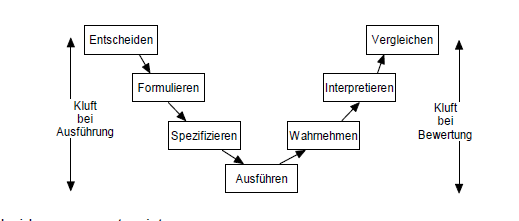
\includegraphics[scale=0.5]{img/phasing.png}
		\caption{Phasen bei Bedienhandlungen}
	\end{figure}
	Kluft der Ausführung = Gulf of Execution; anderes = Gulf of Evalutation (siehe IE)
	
	\item Welche Arten von Handlungsregulation werden unterschieden?
	\begin{itemize}
		\item Bewusst (interlektuelle Ebene): Nutzung des deklarativen Gedäcthnisses, nur eine bewusste interlektuelle Handlung gleichzeitig
		\item Routinehandlung (Ebene der flexiblen Handlungsmuster): automatisiert aus Produktionsgedächtnis; wenige parallel mgl; Auslösung willentlich oder situationsbedingt
		\item Hochautomatisiert (Sensomotorische Ebene): völlig unbewusst, Regelung aus Sinneswahrnehmung und Motorik
	\end{itemize}
	
	\item Wie erfolgt der Umgang mit Fehlern bei Bedienhandlungen?
	\begin{itemize}
		\item Fehler = Abweichung vom Handlungsprozess vom beabsichtigtem Verlauf
		\item Fehlerentdeckung: Verdacht der Abweichung; Entdeckung der Abweichung; Wahrnehmung der Inkongruenz
		\item Fehlerdiagnose: Vergleich mit richtigem Verlauf; Fehlerhypothesen; Interaktionshistorie
		\item Fehlerkorrektur: Direkte Korrektur; Kompensation des Fehlers; Stornierung/Undo
		\item Fehlervermeidung: Minimierung von Gewohnheits-, Bewegungsfehlern durch Hilfen, Lernprogramme, Konzentration auf die Aufgabe\\
		Abfangen von Fehlern durch syntaktische Prüfungen\\
		Vermeidungsstrategien: zb Einschränkung von Freiheitsgraden; Sicherheitsnachfragen
	\end{itemize}
	
	\item Welche Fehlerebenen werden unterschieden?
	\begin{itemize}
		\item Interlektuell: bei Zielen: Denkfehler (zb nicht beachten von Nebenwirkungen)\\
		bei Ausführungsüberwachung: Merk und Vergessensfehler\\
		bei Rückmeldung: Urteilsfehler
		\item Ebene der Handlungsmuster: bei Zielen: Gewohnheitsfehler\\
		bei Ausführungsüberwachung: Unterlassensfehler (zb Überspringen)\\
		bei Rückmeldung: Erkennensfehler (Übersehen, Überhören)
		\item Sensomotorisch: in allen Handlungsprozessen - Bewegungsfehler (Vertippen, Verklicken,..)
	\end{itemize}
	
	\item  Welche Codierungsformen können für die Darstellung von Informationen
	eingesetzt werden?
	\begin{figure}[!h]
		\centering
		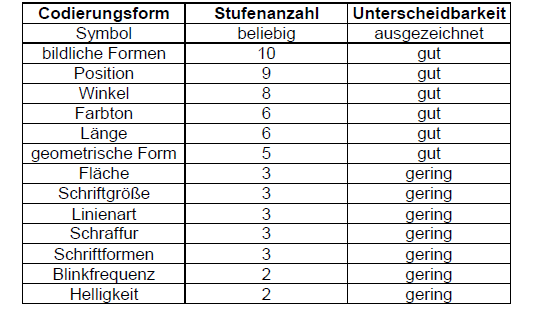
\includegraphics[scale=0.5]{img/codierungsformen.png}
		\caption{Codierungsformen zur Informatiosndarstellung}
	\end{figure}
	\begin{itemize}
		\item sonstiges: (nicht zwingend hierfür relevant, glaub ich)
		\item Hervorheben: Betonung des Rands; Variation der Größe, Isolation,..
		\item besondere Farbe oder Intensität
		\item besonderes Texturmerkmal
		\item Blinken oder Bewegung
	\end{itemize}
	
	\item Welche charakteristischen Eigenschaften sollten zur Darstellung von
	Informationen nach ISO 9241 (Teil 12) beachtet werden?
	\begin{itemize}
		\item Klarheit (schnelle und genaue Vermittlungen des Informationsgehalts)
		\item Unterscheidbarkeit (dargestellte Information kann genau unterschieden werden)
		\item Kompaktheit (nur Informationen die notwendig sind)
		\item Konsistenz (gleiche Information wird stets gleich dargestellt)
		\item Erkennbarkeit (Aufmerksamkeit des Nutzers auf Information lenken)
		\item Lesbarkeit (Information ist gleich zu lesen)
		\item Verständlichkeit (Bedeutung ist leicht verständlich, eindeutig, interpretierbar und erkennbar)
	\end{itemize}
	
	\item Was ist beim Einsatz von Textfonts zu beachten?
	\begin{itemize}
		\item ausreichend groß und gut lesbar
		\item keine Kursivschreibung (Probleme bei schrägen Linien bei niedriger Auflösung) und keine Großschreibung(d.h. ALLE BUCHSTABEN GROß :-) )
		\item optimal: Serifenschrit
		\item Zeilenlänge = 20fache der Schriftgröße
		\item sinnvoller Zeilenabstand
		\item nach ISO 9241 (Auszug)
		\item Zeichenbreite abhängig von Zeichenhöhe
		\item Wortabstand mindestens ein Zeichen groß
		\item max Anzahl Zeichen pro Zeile = 60
	\end{itemize}
	
	\item Wozu lässt sich Gruppierung nutzen und wie kann sie umgesetzt werden?
	\begin{itemize}
		\item Elemente mit Sinnzusammenhang in Gruppen zusammenfassen
		\item Elemente mit ähnlichem Aussehen
		\item Elemente in Gruppe entsprechend des Arbeitsablaufes darstellen
		\item für Suchen und Vergleichen: Elemente der Gruppe in Spalte anordnen
		\item Überschriften und Rahmen erhöhen Übersicht
		\item Umsetzung: Gruppierung nach fachlichen Kriterien
		\item zusammengehörige Informationen auf Maske sollten deutlich, auch räumlich, zusammen angeordnet sein
		\item Fluchtlinien minimieren -> Ausrichtung aller Elemente an wenigen Fluchtlinien
	\end{itemize}
\end{enumerate}

\subsection{Normen und Bildschirmarbeit}
\begin{enumerate}
	\item Was beinhaltet ISO 9241-Teil 110 Grundsätze ergonomischer Dialoggestaltung?
	\begin{itemize}
		\item Dialogrichtlinien
		\item unabhängig von bestimmten Dialogtechniken
		\item liefert ergonomische Gestaltung von interaktiven Systemen und
		\item \textit{Grundsätze der Dialoggestaltung:}
		\item Aufgabenangemessenheit: System unterstützt User beim Erledigen seiner Aufgabe, d.h. Funktionalität ist an Aufgabenbereich angepasst
		\item Selbstbeschreibungsfähigkeit: muss für Nutzer offensichtlich sein zu jeder Zeit zu erkennen wo er sich im Dialog befindet, welche Handlungen unternommen werden können
		\item Steuerbarkeit: Dialogablauf: starten, Richtung und Geschwindigkeit beeinflussbar durch User
		\item Erwartungskonformität: entspricht allgemein anerkannten Konventionen und aus Nutzerkontext vorhersehbare Benutzerbelange
		\item Fehlertoleranz: Arbeitsergebnis kann trotz erkennbar fehlerhafter Eingaben mit minimalen Aufwand seitens des Benutzers erreicht werden
		\item Individualisierbarkeit: HCI und Darstellung von Informationen kann durch Nutzer angepasst werden
		\item Lernförderlichkeit: unterstützt Nutzer beim Erlernen des Systems\\
		\\
		\item Anwendung der Grundsätze  unter Berücksichtigung der Benutzermerkmale: \\
		Aufmerksamkeitsspanne; Grenzen des Kurzzeitgedächtnisses\\
		Lerngewohnheiten, Grad an Erfahrun bzgl Arbeit und Umgang mit Dialogsystems\\
		mentales Modell des Nutzers bzgl des Dialogsystems
		\item Grundsätze sind nicht unabhängig voneinander -> Priorisieren der Grundsätze nach Zielen der Organsitation; Benutzerbelange; zu unterstützende Aufgaben
	\end{itemize}
	
	\item Wie erreiche ich ...
	\begin{itemize}
		\item Selbsterklärungsfähigkeit? angezeigte Informationen sollten handlungsbegleitend sein; minimierte Notwendigkeit von Handbüchern (oder anderen externen Hilfen); Informierung über Änderung des Zustands; Überblick über die nächsten Dialogschritte; 
		\item Aufgabenangemessenheit? zeige nur Informationen an, die im Zusammenhang mit der Aufgabe stehen (Bsp: Einhaltung zeitkritischer Bearbeitung -> einzuhaltende Termine zuerst anzeigen); Form der Ein/Ausgabe sollte zu Aufgabe passen; Dialogschritte sollten zum Arbeitsablauf passen
		\item Steuerbarkeit? Geschwindigkeit durch Nutzer und nicht durchs System vorgeben; Steuerung der anzuzeigenden Datenmenge; Unterbrechen und Wiederaufnehmen des Dialogs ermöglichen; Elemente zur Navigation durch den Dialog bereitstellen 
		\item Erwartungskonformität? Vokabular der Aufgabe verwenden; Verhalten und Darstellung innerhalb einer Aufgabe/ähnlichen Aufgaben konsistent; Formate an kulturelle und sprachliche Konventionen anpassen -> Bsp: Symbole für Öffnen, Neu, Speichern -> gleiches Verhalten wie in bekannten Tools
		\item Fehlertoleranz? Fehler dem Nutzer anzeigen; Verbesserungsvorschläge anbieten; über automatische Korrektur von Fehler informieren; Überprüfung der Eingabe von Fehlern VOR Verarbeitung; Verhinderung von Systemabstürzen
		\item Individualisierbarkeit? Techniken zur Anpassung an charakteristische Eigenschaften des Nutzers; zb Farbschema auswählen; Umfang von Erläuterungen (zb Hilfeinformationen) an Nutzer bzw dessen Wissen anpassbar; Format und Typ der Ein/Ausgabe änderbar; Reset auf Werkseinstellungen mgl; 
		\item Lernförderlichkeit? Rückmeldungen und Erläuterungen nutzen; minimale Eingabe von Informationen, aber zusätzliche Informationen auf Anforderung liefern; Regeln und zugrundeliegende Konzepte dem Nutzer zugänglich machen
	\end{itemize}
	
	\item Wie lässt sich Gebrauchstauglichkeit messen?\\
	in 4 Aspekten
	\begin{itemize}
		\item \textbf{Effektivität}: Genauigkeit und Vollständigkeit, mit der Benutzer ein bestimmtes Ziel erreichen 
		\item \textbf{Effizienz}: Der im Verhältnis zur Genauigkeit und Vollständigkeit eingesetzte Aufwand zum Erreichen des Ziels
		\item \textbf{Zufriedenstellung}: Freiheit von Beeinträchtigungen und positive Einstellungen ggüber der Nutzung des Produkts
		\item \textbf{Nutzungskontext}: Benutzer, Arbeitsaufgaben, Arbeitsmittel, physische und soziale Umgebung
	\end{itemize}
	1-3 werden im Rahmen des Nutzungskontextes betrachtet
	
	\item Nennen sie Kriterien zur Messung der Gebrauchstauglichkeit!\\
	siehe eine Frage vorher(?)
	
	\newpage
	\item Was lässt sich messen bei der Gebrauchstauglichkeit? (allgemein)
	\begin{table}[!h]
		\centering
		\begin{tabular}{|p{13em}|p{13em}|p{13em}|}
			\hline
			\textbf{Maß der Effektivität} & \textbf{Maß der Effizienz} & \textbf{Maß der Zufriedenstellung}\\
			\hline
			Grad der Zielerreichung in \% & Zeit für Erledigung einer Aufgabe & Einstufungsskala der Zufriedenheit\\
			\hline
			\%-Satz der Nutzer die Aufgabe erfolgreich abschließen & Abgeschlossene Aufgaben je Zeiteinheit & Häufigkeit freiwilliger Nutzung\\
			\hline
			Durchs. Genauigkeit der abgeschlossenen Aufgaben & Monetäre Kosten der Aufgabenerledigung & Häufigkeit von Beschwerden\\
			\hline
		\end{tabular}
	\end{table}
	
	\item Ein Dialogsystem soll angemessen für geübte Benutzer sein! Welche Usability-
	Messungen sind sinnvoll?
		\begin{table}[!h]
			\centering
			\begin{tabular}{|p{13em}|p{13em}|p{13em}|}
				\hline
				\textbf{Maß der Effektivität} & \textbf{Maß der Effizienz} & \textbf{Maß der Zufriedenstellung}\\
				\hline
				Anzahl ausgeführter Aufgaben hoher Schwierigkeit & Effizienz im Verhältnis zu einem Experten-Benutzer & Einstufungsskala für Zufriedenstellung mit Produktmerkmalen für hohe Ansprüche\\
				\hline
				Prozentsatz relevanter Funktionen, die genutzt werden&&\\
				\hline
			\end{tabular}
		\end{table}
	\item Wie kann der Nachweis der Gebrauchstauglichkeit für Software geführt werden?
	\begin{itemize}
		\item 	mit dem ErgoNorm-Prüfverfahren; Verifikation sehr teuer, daher Falsifizierbarkeitsansatz (Software ist richtig bis Gegenbeweis)
		\item zweiteiliges Prüfverfahren:
		\begin{enumerate}
			\item Benutzerfragebogen -> Untersuchung von Nutzerproblemen
			\item Prüfverfahren: Anforderungsentwicklung und Normkonformitätstest sowie Erhärtungsprüfung für vermutete Normabweichungen -> Methoden: Aufgabenanalyse mittels Szenarien; Inspektion; Dokumentanalyse,..
		\end{enumerate}
		\item Definition von Prüfkriterien: Nutzungskontext ---erkennen der--> Erfordernisse ---ableiten der---> Anforderungen ---transformieren in---> Prüfkriterien
		\newpage
		\item \textbf{Erhärtungsprüfung:}
		\begin{figure}[!h]
			\centering
			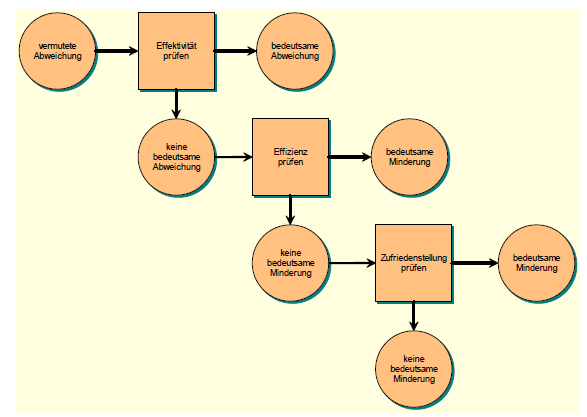
\includegraphics[scale=0.5]{img/erhaertungspruefung.png}
			\caption{Entscheidungsregeln bei Erhärtungsprüfung}
		\end{figure}
		\item \textbf{Nonkonformitätsprüfung:}
		\begin{figure}[!h]
			\centering
			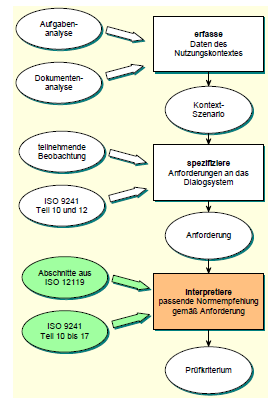
\includegraphics[scale=0.5]{img/nonkonformitaet.png}
			\caption{Nonkonformitätsprüfung}
		\end{figure}
		\begin{itemize}
			\item ISO Teil 10 Dialogprinzipien; Teil 12 Informationsdarstellung
		\end{itemize}
	\end{itemize}

	\item Was regelt die Bildschirmarbeitsverordnung?
	\begin{itemize}
		\item Vorschriften zur Vorsorge, zum Arbeitsablauf und zu Pausen für alle Beschäftigten
		\item gilt nicht für öffentliche EDV Geräte; Rechenmaschinen, Kassen mit kleiner Datenanzeige, Bildschirme für Videoüberwachung,....
		\item Mindestanforderungen für Arbeitsplatzgestaltung: \\
		Arbeitsmittel: Bildschirm, Tastatur, Tisch und Stuhl\\
		Arbeitsumgebung: Bewegungsraum, Licht, Lärm, Klima, Strahlung\\
		Zusammenwirken Mensch-Arbeitsmittel: Software und Arbeitsaufgaben
		\item Anforderungen an Körperhaltung: \\
		optimaler Abstand zum Gerät: 90cm; optimale Blickrichtung\\
		großer Greifraum
		\item Arbeitstätigkeit am Bildschirm regelmäßig durch andere Tätigkeiten oder Pausen unterbrechen
		\item Prüfsiegel für Geräte
		\item Anforderungen an Bildschirme: \\
		Ergonomie: gleichmäßige Beleuchtung; Kontrast; Flimmerfrei,..\\
		Emissionen: magnetische Störungen dürfen kein Flackern verursachen\\
		Ökologie: geringer Energieverbrauch; Recyclebar,...
	\end{itemize}
	
	\item Wie kann die Einhaltung von Ergonomie-Normen geprüft werden?\\
	müsste zwei Fragen vorher das ErgoNorm Verfahren sein
\end{enumerate}

\subsection{Fenstersysteme}
\begin{enumerate}
	\item Welche Begriffe/Konzepte werden neben Fenstern bei
	modernen Fenstersystemen noch benötigt?
	\begin{itemize}
		\item Window: Ausgabefläche, die zu platzieren ist
		\item Desktop/Workspace: Fläche auf dem Fenster platziert werden
		\item Display: Verwaltung der Ausgabefläche und Eingabegeräte
		\item Screen: physisch vorhandener Bildschirm
		\item Virtual Screen/Workspace/Desktop: Durch Speicherabbildung vorhandener Platz aus dem aktuelle Ausschnitte eingeblendet werden können
	\end{itemize}
	
	\item Fenstersysteme – Strategien zur Platzierung von Fenstern
	\begin{itemize}
		\item \textbf{Compositing}: Fenster werden erst erstellt, separat gemalt und dann zusammengepackt um sie in verschiedenen 2D oder 3D Umgebungen darzustellen
		\item \textbf{Stacking:} Fenster können überlappend dargestellt werden indem Hintergrundfenster zuerst gezeichnet werden; darf nicht als Composition Manager deklariert sein
		\item \textbf{Tilling}: nicht überlappend; Fenster werden neben- oder unter/übereinander dargestellt
		\item \textbf{Dynamic:} switchen dynamisch zw. stacking und tilling
	\end{itemize}	
	
	\newpage
	\item Erläutern Sie das Schichtenmodell eines Fenstersystems!
	\begin{figure}[!h]
		\centering
		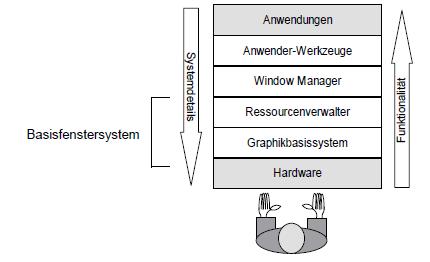
\includegraphics[scale=0.7]{img/window_layers.png}
		\caption{Schichtenmodell eines Fenstersystems}
	\end{figure}
	\begin{itemize}
		\item \textbf{Anwenderwerkzeuge}
		\begin{itemize}
			\item Typische Dialogbausteine müssen nicht für jede Applikation neu implementiert werden (Toolkits)
			\item Schnittstelle zw Anwendung und Fenstersystemfunktionalität
			\item typischerweise sind Bibliotheken die Anwenderwerkzeuge
		\end{itemize}
		\item \textbf{Window Management}
		\begin{itemize}
			\item Anzeige verschiedener Applikationen auf dem Bildschirm; Dialogmöglichkeiten auf Sitzungsebene
			\item zuständig für Aussehen und Verhalten
			\item sorgt für Positionierung und die Ausstattung der Fenster
			\item liefert Standardtechniken, mit denen der Benutzer interagieren kann (zb Close Button)
			\item Bildschirmaufteilung: Wo ist noch Platz? Welche Anwendung ist ikonifiziert?
			\item Sitzungsverwaltung: Navigation zw. Applikationen; Menutechnik; Fensterrahmen,...
			\item verschiedene Window Manager: siehe Frage vorher
			\item 
		\end{itemize}
		\item \textbf{Ressourcen Verwaltung}
		\begin{itemize}
			\item Konkurrierender Zugriff auf Ressourcen; Synchronisation zw Applikationen
			\item für $k$ Terminals (Monitor, Eingabegeräte) gibt es genau eine Instanz eines Fenstersystems; Dazu $n$ Anwendungen mit je $m$ Fenstern
			\item Elementare Konzepte:
			\item Objekt ''Fenster'': Zustand (Sichtbarkeit, (in)aktiv); Größe; Fußpunkt (Darstellung auf Screen)
			\item Objekt ''Ereignis'': Eventtyp; Timestamp; Ort; zugehöriges Fenster
			\item Objekt ''Font''
			\item Objekt ''Graphikkontext''
			\item Objekt ''Farbtabelle''
		\end{itemize}
		\item \textbf{Graphikbasissystem}
		\begin{itemize}
			\item Realisiert Ausgabefunktionalität für Fenstersysteme (2D-Rastergrafik); hardwarenah angelegt für hohe Ausgabegeschwindigkeit
			\item Elementare Konzepte - 2D:
			\item Zeichenfläche - Fenster (Drawable):\\
			Ebenenformat - XY Koordinaten; Tiefe: Z-Format
			\item Ausgabe-Objekte und grafische Kontexte:\\
			Linien- oder Flächenprimitive, Textausgabe
			\item Gedächtnis der Ausgabe:\\
			Daten-gepufferte Ausgabe (Ausgabe in Hintergrundspeicher, anschließend Teile auf Bildschirm kopieren)\\
			Bearbeiten und Vergessen: Rasterkonvertierung und dann Ausgabe
			\item Events und Warteschlange:\\
			Umwandlung gerätespez. Events und Speicherung in Queue (log. Bildkoords, Timestamp, Eventcode)
		\end{itemize}
		\item \textbf{Hardware}
		\begin{itemize}
			\item Rasterbildschirm mit Grafikprozessor, Maus, Tastatur, Multimediakomponenten
		\end{itemize}
	\end{itemize}
	
	\item Was sind Widgets und nennen sie typische Elemente in
	Widgetbibliotheken?
	\begin{itemize}
		\item Widget = Dialogbaustein (heute auch kleine Anwendungen bei Android/Win 7)
		\item in Motif: 
		\item Primitive Widgets: Dialogbausteine mit Darstellung und Interaktion (Buttons,..)
		\item Composite Widgets: Dialogbausteine zur Anordnung von Elementen (LayoutManager)
		\item Shell Widgets: Dialogbausteine zum Behandeln neuer Fenster (Fenster, Dialogboxen)
	\end{itemize}
	
	\item Welche Probleme treten bei der Anbindung von Funktionalität in objektorientierten Sprachen auf?
	\begin{itemize}
		\item Implementierung  oft in C (da OS-nah)
		\item Fenstersystem vom Prinzip her aber OO
		\item Probleme:
		\item Widgets: Widget in C++ Wrapper einschließen\\
		Problem: C++Instanz ex. bevor Widget dargestellt wird; Unklar wann Ressourcen in Unterklassen das Widget beeinflussen; Eventanbindung
		\item Eventanbindung: Events durch Callbacks realisiert, CB benötigt Referenz auf Widget (siehe oben Wrapper vor Widget initialisiert)\\
		Lösung: 1. CB als globale Funktion;\\
		2. statische Memberfunktionen 
	\end{itemize}
	
	\item Welche Vorteil bietet ''Markup and Code-Behind'' gegenüber herkömmlicher Benutzungsoberflächenprogrammierung?
	\begin{itemize}
		\item Markup+Code-Beding: Trennung der Oberfläche und Anwendungslogik
		\item dadurch können Designer und Entwickler parallel arbeiten
		\item einfacher Austausch der Komponenten
	\end{itemize}
	
	\item Nennen Sie Bibliotheken zur Gestaltung graphischer
	Benutzungsoberflächen und vergleichen sie diese!
	\begin{table}[!h]
		\centering
		\begin{tabular}{|p{13em}|p{13em}|p{13em}|}
			\hline
			\textbf{GTK+} & \textbf{QT} & \textbf{WPF}\\
			\hline
			Signals and Slots als Eventhandling & Signals and Slots als Eventhandling&\\
			\hline
			in C mit C++Wrapper für OO; vorrangig für X-Window& plattformübergreifend; C++ & für Windows ab Vista; setzt auf DirectX \\
			\hline
			besteht aus Teilbibliotheken & & Oberfläche 2D, Fenster Ikonen in 3D\\
			\hline
			&& Markup and Code Behind\\
			\hline
		\end{tabular}
	\end{table}
	weitere: Java -> AWT; Swing;SWT
\end{enumerate}

\subsection{Dialogtechniken}
\begin{itemize}
	\item Was sind Interaktions- und Dialogtechniken?
	\begin{itemize}
		\item Interaktionstechnik = Realisierung einer Interaktionsaufgabe\\
		Charakterisierung durch die zu lösende Aufgabe und zu welchem Interaktionsstil sie angehören\\
		Interaktionsaufgabe = bestimmte Aktion, die wiederholt oder in ähnlicher Form auftreten
		\item wiederkehrende Dialogmuster durch sog. Interaktionsformen beschreiben und realisieren\\
		Interaktionsform = festgelegt Auswahl von Ein/Ausgabevorgängen zsm mit ihren Abfolgebedingungen, die zu stereotypischen Kommunikationssequenzen führen
		\item \textit{typische Techniken}:
		\item natürliche Sprache: Anwendung in KI, Syntaktische und Semantische Analyse; Sprachein/ausgabe
		\item Frage-Antwort-Dialoge: System fragt; Nutzer antwortet
		\item Kommandodialog: veränderter Frage-Antwort; Nutzer stellt System jetzt Kommandos (klassisch bash ;-))
		\item Menügesteuerter Dialog: 
		\item Formulardialog: quasi nachgebildetes Papierformular
		\item Direkte Manipulation
		\item Graphischer Dialog
		\item Fenstertechnik - WYSIWYG
		\item heute durch Fenstersysteme: Kopplung unterschiedlicher Stile
	\end{itemize}
	\item Vergleichen Sie PullDown mit Popup-Menüs!
	\begin{table}[!h]
		\centering
		\begin{tabular}{|l|p{15em}|p{15em}|}
			\hline
			&\textbf{Pulldown} & \textbf{Popup}\\
			\hline
			&klappt unter Titel auf nachdem Titel angeklickt wurde; verschwindet nach Auswahl oder bewegen des Cursors außerhalb der Menufläche & unsichtbares Menu; erscheint an Cursorposition\\
			\textbf{Bsp} &klassische Menuleiste & Contextmenu\\
			\hline			
			\textbf{Vorteile} & Darstellung: ständiger Hinweis auf Steuerungsmglkeiten durch Menuleiste & Mauseinsatz: Minimierung der erforderlichen Mausbewegung\\
			& Wirkungsbreite: Optionen können über mehrere Bildschirmbereiche wirken & \\
			& Raumbedarf: relativ gering aufm Bildschirm& Raumbedarf: Nutzfläche bleibt vollständig erhalten\\
			\hline
			\textbf{Nachteile} & Optionenmenge: nur beschränkte Auswahl von Optionen mgl & Optionenmenge: nur geringe Anzahl von Optionen mgl \\
			& Mauseinsatz: längere Mausbewegungen erforderlich & Wirkungsbreite: Aktionen sind objektbezogen\\
			&&Darstellung: Steuerungsmglkeiten erst nach Öffnen sichtbar \\
			\hline
		\end{tabular}
	\end{table}
	Standardelemente des Fenstersystems
	\item Beschreiben Sie Varianten von Menüs!
	\begin{itemize}
		\item Binäres Menü: genau zwei auswählbare Elemente
		\item Erweitertes Menü: Menu in Seiten untergliedert
		\item Einfach/Mehrfac-Menu: Nutzer kann genau/mehr als eine Wahl treffen
		\item Permanentes Menu: ständig auf Bildschirm sichtbar
		\item Pulldown/Popup: siehe oben
		\item Drop-Down: Menu klappt unter Titel auf nachdem der Titel berührt wurde; verschwindet auch wieder
		\item Tear-Off: 
	\end{itemize}
	\newpage
	\item Welche Vor- und Nachteile haben spezielle Dialogtechniken (Sprache, Menü, Formular)?
	\begin{table}[!h]
		\centering
		\begin{tabular}{|l|p{13em}|p{13em}|p{13em}|}
			\hline
			&\textbf{Natürliche Sprache} & \textbf{Menü} & \textbf{Formular}\\
			\hline
			\hline
			\textbf{Vorteile} & einfach anwendbar & vollständige Führung des Nutzers durchs System & explizit Werte in Maske eintragen\\
			& mächtig genug, um jede Anfrage zu übermitteln & einfacher Auswahlmechanismus & Navigation zw Eingabefeldern\\
			& keine Formale Sprache erlernen &schnell bei kleinen Wertemengen& Vertrautheit bei Formularen, die Papier entsprechen\\
			\hline
			\textbf{Nachteile} & derzeit nur Verarbeitung von Teilmenge der Sprache & langatmiger Dialog bei großer Auswahlmöglichkeit& Masken oft mit Informationen überladen\\
			& Benutzer überschätzen Fähigkeiten des Systems &Mehrdeutigkeit der Zuordnung (wo finde ich was?)& Probleme, wenn alle Felder ausgefüllt werden müssen\\
			& Komplexe Sachverhalte oft nur umständlich zu formulieren &Wie lange Menu sichtbar?& Layoutgestaltung (Prinzipien der Wahrnehumgslehre)\\
			& oft Mehrdeutigkeiten && \\
			\hline
		\end{tabular}
	\end{table}
	\item Welche Aufgabe hat ein Layoutmanager!
	\begin{itemize}
		\item Anordnung der Kindelemente nach bestimmten Kriterien
	\end{itemize}
	\item Nennen sie typische Beispiele für Layoutmanger!
	\begin{itemize}
		\item Lineare: Kinder nacheinander in Reihenfolge der Richtung (vertical/horizontal) eingeordnet
		\item tabellarisch: 
		\item Anordnung in Rubriken (zb BorderLayout Java)
		\item Anordnung mit Hilfe von Contraints
		\item Baum- oder Graphenalgorithmen
	\end{itemize}
	
	\item Nennen sie 3D Interaktionstechniken?\\
	Trackball (= §D Hülle um Objekt)\\
	Semitransparente Volumina als 3D Cursor\\
	Anfassbare pyhsische Objekte (zb Linse auf Tabletop)
	
	\item Welche Möglichkeiten hat man zur „Erweiterung“ der Zeichenfläche?\\
	Nutzen mehrerer, alternativer Zeichenflächen (Card-Layout, Tab-Layout)\\
	Scrollbars (Verschieben des darstellbaren Bereichs)\\
	ZUIs
	
	\item Was ist direkte Manipulation?\\
	\begin{itemize}
		\item Prinzipien:
		\item permanente Sichtbarkeit der jeweils interessierenden Objekte
		\item schnelle, umkehrbare Operationen, deren Wirkung unmittelbar sichtbar werden
		\item physische Aktionen, wie Bewegen eines Zeigegerätes, Selektionsmechanismen
		\item generische Kommandos und Funktionsobjekte (Mülleimer, Printer)
		\item OO Interaktionssyntax: erst Auswahl Objekt, dann Methoden/Kommandoauswahl
		\\\\
		\item Vorteile:
		\item schnell erlernbar (für Anfänger); effizient (für Experten)
		\item kaum Fehlermeldungen notwendig
		\item Probleme:
		\item leistungsfähige Zeigeinstrumente notwendig
		\item hoher Programmieraufwand
	\end{itemize}
	\item Wie würden sie Menüs an einer Powerwall nutzen? Ziele der Interaktion?\\
	PopupMenu mit am sinnvollsten; DropDown mit ShortCuts auch sinnvoll mgl\\
	\item Welche Gesten/Interaktionsgeräte sind sinnvoll einsetzbar an Powerwall?\\
	Eyetracker; Tracker für Bewegung des Körpers (Bsp Wii)
	
	\item Welche Gesten halten sie für sinnvoll zum Ersatz von „arm“ und „activate“ auf eine Touchscreen?
\end{itemize}

\subsection{Metaphern}
\begin{itemize}
	\item Was ist eine Metapher ?
	\begin{itemize}
		\item sprachliches Bild
		\item Dadurch wird auf die Ähnlichkeit der Begriffe in einem speziellen Kontext hingewiesen
		\item Metaphern nutzen die Vertrautheit eines Begriffes, um ein Konzept	anschaulich zu machen – positive Analogien.
		\item Metaphern können Ordnung und Struktur in Schnittstellen bringen bei orientierung an Nutzer vertraute Konzepte \\
		Bsp: Desktop-Metapher; Buch-Metapher; Reise-Metapher (''erst Aufgabe erledigen bevor ich weiter kann''); Raum-Metapher (zb in Informationssystemen)
	\end{itemize}
	
	\item Wie lassen sich Metaphern bei der Arbeit mit Dialogsystemen sinnvoll nutzen?\\
	siehe vorher Punkt 3
	
	\item Ein Entwurfsmuster beschreibt ein bestimmtes, in einem
	bestimmten Kontext immer wiederkehrendes Entwurfsproblem
	sowie ein generisches Schema zur Lösung dieses Problems.
	
	\item Wozu dient das Entwurfsmuster Fassade?
	\begin{itemize}
		\item einheitliches Interface für Menge von Klassen in einem Subsystem 
		\item ermöglicht dadurch leichtere Nachnutzung des Subsystems
		\item Anwendbarkeit: einfache Schnittstelle zu komplexen Subsystemen (zb WidgetBibliothek)
		\item Entkopplung des Systems und Aufteilung in Schichten
	\end{itemize}
	
	\item Wozu dient das Entwurfsmuster Kompositum(Composite)?
	\begin{itemize}
		\item Zusammenfügen von Objekten in baumartigen Strukturen, um Teile-Ganzes-Hierarchie zu repräsentieren
		\item Teilnehmer: Client - manipuliert Objekte durch Schnittstelle von Komponente\\
		Blatt: repräsentiert Kindobjekt, definiert Verhalten für primitive Objekte\\
		Komponenten: deklariert Schnittstelle für Objekte in Struktur und Zugriff auf Kindobjekte
		\item Kompositum: definiert Verhalten für Komponenten, die Kindobjekte haben können
	\end{itemize}

	\item Wozu dient das Entwurfsmuster Dekorierer (auch Wrapper)?
	\begin{itemize}
		\item Dynamisches Hinzufügen zusätzlicher Verantwortlichkeiten
		\item flexible Alternative zur Unterklassenbildung existierender Funktionalität bereit
	\end{itemize}
	
	\item Wozu dient das Entwurfsmuster Observer?
	\begin{itemize}
		\item Definition einer 1:n Abhängigkeit zw Objekten um bei Änderung des einen Objektes alle n abhängigen Objekte zu informieren
	\end{itemize}
	
	\item Wozu dient das Entwurfsmuster ...?\\
	Singleton, Abstract Factory; Command; Adapter; Bridge; Proxy
	
	\item Vergleichen Sie das Entwurfsmuster Observer mit dem Model-View-Controller-Modell!
	\begin{itemize}
		\item Observer = Pattern | MVC = Architektur
		\item Observer kann im MVC benutzt um effizient die Änderung mitzuteilen
	\end{itemize}
\end{itemize}
